\documentclass[12pt,a4paper]{article}

\usepackage[utf8]{inputenc}
\usepackage[T1]{fontenc}
\usepackage[english]{babel}
\usepackage{graphicx}
\usepackage{float}
\usepackage{hyperref}
\usepackage{geometry}
\usepackage{listings}
\usepackage{tikz}
\usepackage{xcolor}
\usetikzlibrary{shapes.geometric,positioning}
\usetikzlibrary{arrows.meta, positioning}

\geometry{margin=2.5cm}

% Listings
\lstset{
    frame=single,
    basicstyle=\ttfamily\small,
    captionpos=b,
    numbers=left,
    numberstyle=\tiny,
    breaklines=true,
    tabsize=4
}

\renewcommand{\lstlistingname}{Listing}
\renewcommand{\lstlistlistingname}{List of Listings}

\begin{document}

% Title page
\begin{titlepage}

\begin{minipage}{0.5\textwidth}
    \flushleft
    \IfFileExists{imgs/prz_ang.png}
    {\includegraphics[height=2.5cm]{imgs/prz_ang.png}}
    {\fbox{\parbox[c][2.5cm][c]{5cm}{\centering University logo}}}
\end{minipage}
\begin{minipage}{0.5\textwidth}
    \flushright
    \IfFileExists{imgs/weii_ang.png}
    {\includegraphics[height=2.5cm]{imgs/weii_ang.png}}
    {\fbox{\parbox[c][2.5cm][c]{5cm}{\centering Faculty logo}}}
\end{minipage}

\vspace{3cm}

\begin{center}

{\Large \textbf{Machine Learning}}

\vspace{1cm}

{\LARGE \textbf{Project Report}}

\vspace{1cm}

{\large title: ``Product Price Prediction Based on the Myntra Catalog''}

\end{center}

\vfill

\begin{minipage}{0.5\textwidth}
\flushleft
\textbf{Date:} 15.06.2026
\end{minipage}
\begin{minipage}{0.5\textwidth}
\flushright
\textbf{Group:} LX \\
Arman
\end{minipage}

\end{titlepage}

% Lists

\tableofcontents
\newpage

\listoffigures
\newpage

\listoftables
\newpage

\lstlistoflistings
\newpage

% Content

\section{Project Goal}

The goal of this project was to build a machine learning system for predicting product prices in Indian rupees using data from the Myntra product catalog. The work was organized as a small Python project, not only as a notebook. It includes separate modules, a training pipeline, saved models, metric reports, and a Streamlit application where the prediction can be tested manually.

The dataset contains basic product information such as brand, gender category, number of images, primary color, product description, and price. The target variable is the column \texttt{Price (INR)}. This is a regression problem, because the model returns a numerical value: the estimated product price.

The practical goals of the project were:
\begin{itemize}
    \item to prepare the data for model training,
    \item to compare several regression algorithms,
    \item to make the result available through a simple web application.
\end{itemize}

\section{Dataset Description}

The source dataset is stored in the project under the following path:

\begin{lstlisting}[language=bash, caption={Dataset location}]
data/raw/myntra_products_catalog.csv
\end{lstlisting}

The dataset contains 12491 rows and 8 columns. The most important columns used in the project are shown in Table~\ref{tab:data}.

\begin{table}[H]
\centering
\begin{tabular}{|p{4cm}|p{9cm}|}
\hline
\textbf{Column} & \textbf{Meaning} \\ \hline
\texttt{ProductBrand} & product brand \\ \hline
\texttt{Gender} & product category, for example Men, Women, Boys, Unisex \\ \hline
\texttt{NumImages} & number of product images in the catalog \\ \hline
\texttt{PrimaryColor} & main product color \\ \hline
\texttt{Description} & text description of the product \\ \hline
\texttt{Price (INR)} & real product price in Indian rupees \\ \hline
\end{tabular}
\caption{Main columns used in the project}
\label{tab:data}
\end{table}

Before training the models, the target price was transformed using \texttt{log1p}. This is useful for price data, because prices often have a wide range and a few expensive products can strongly affect the model. After prediction, the result is transformed back with \texttt{expm1}, so the application shows a normal price in INR.

\subsection{Exploratory Data Analysis Plots}

During the first analysis, the price distribution was checked after logarithmic transformation. This plot is useful because the original price column is strongly skewed. After applying \texttt{log1p}, the distribution becomes easier for regression models to learn.

\begin{figure}[H]
\centering
\IfFileExists{imgs/eda_price_plots.png}
{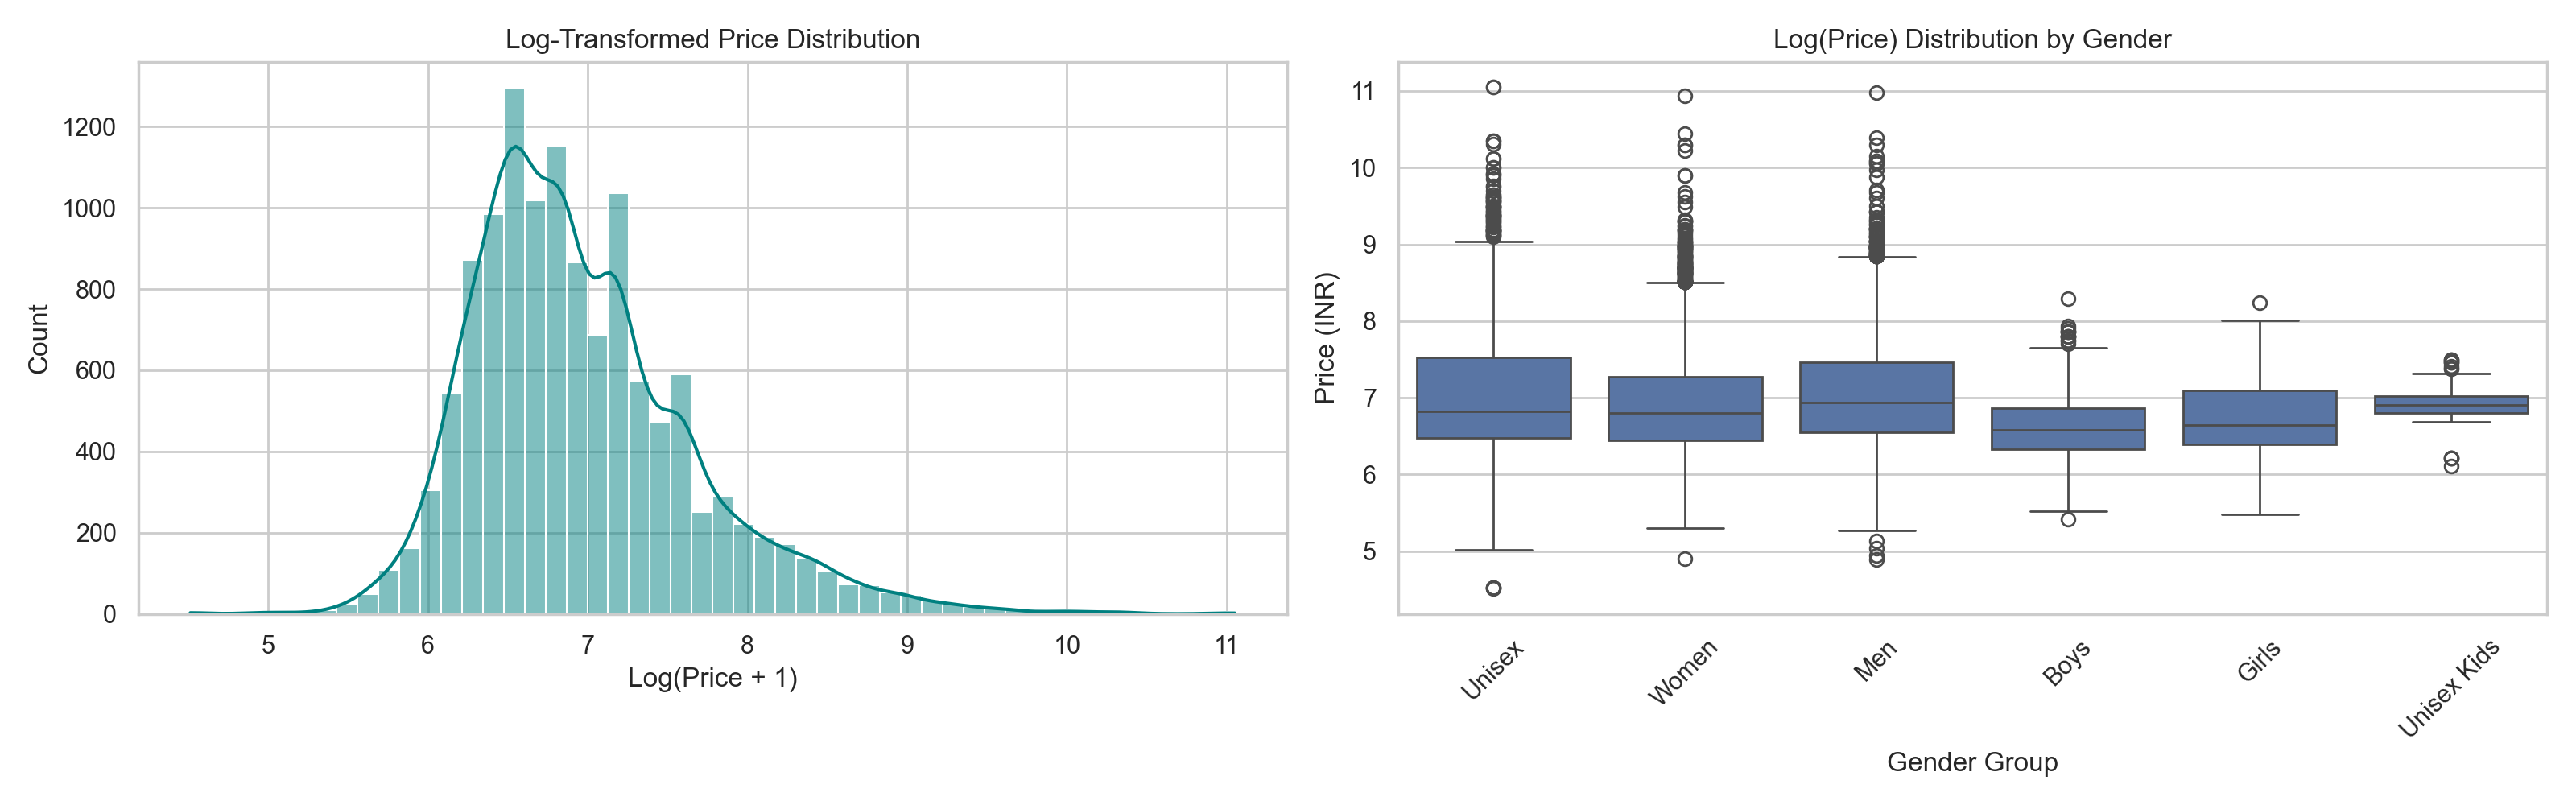
\includegraphics[width=0.95\textwidth]{imgs/eda_price_plots.png}}
{\fbox{\parbox[c][6cm][c]{0.95\textwidth}{\centering Missing image: \texttt{imgs/eda\_price\_plots.png}}}}
\caption{Exploratory plots: log-transformed price distribution and log-price distribution by gender}
\label{fig:eda_price_plots}
\end{figure}

For easier use in the report, the same two charts are also saved as separate image files. The histogram is stored as \texttt{log\_price\_distribution.png}, and the gender boxplot is stored as \texttt{log\_price\_by\_gender.png}.

\begin{figure}[H]
\centering
\IfFileExists{imgs/log_price_distribution.png}
{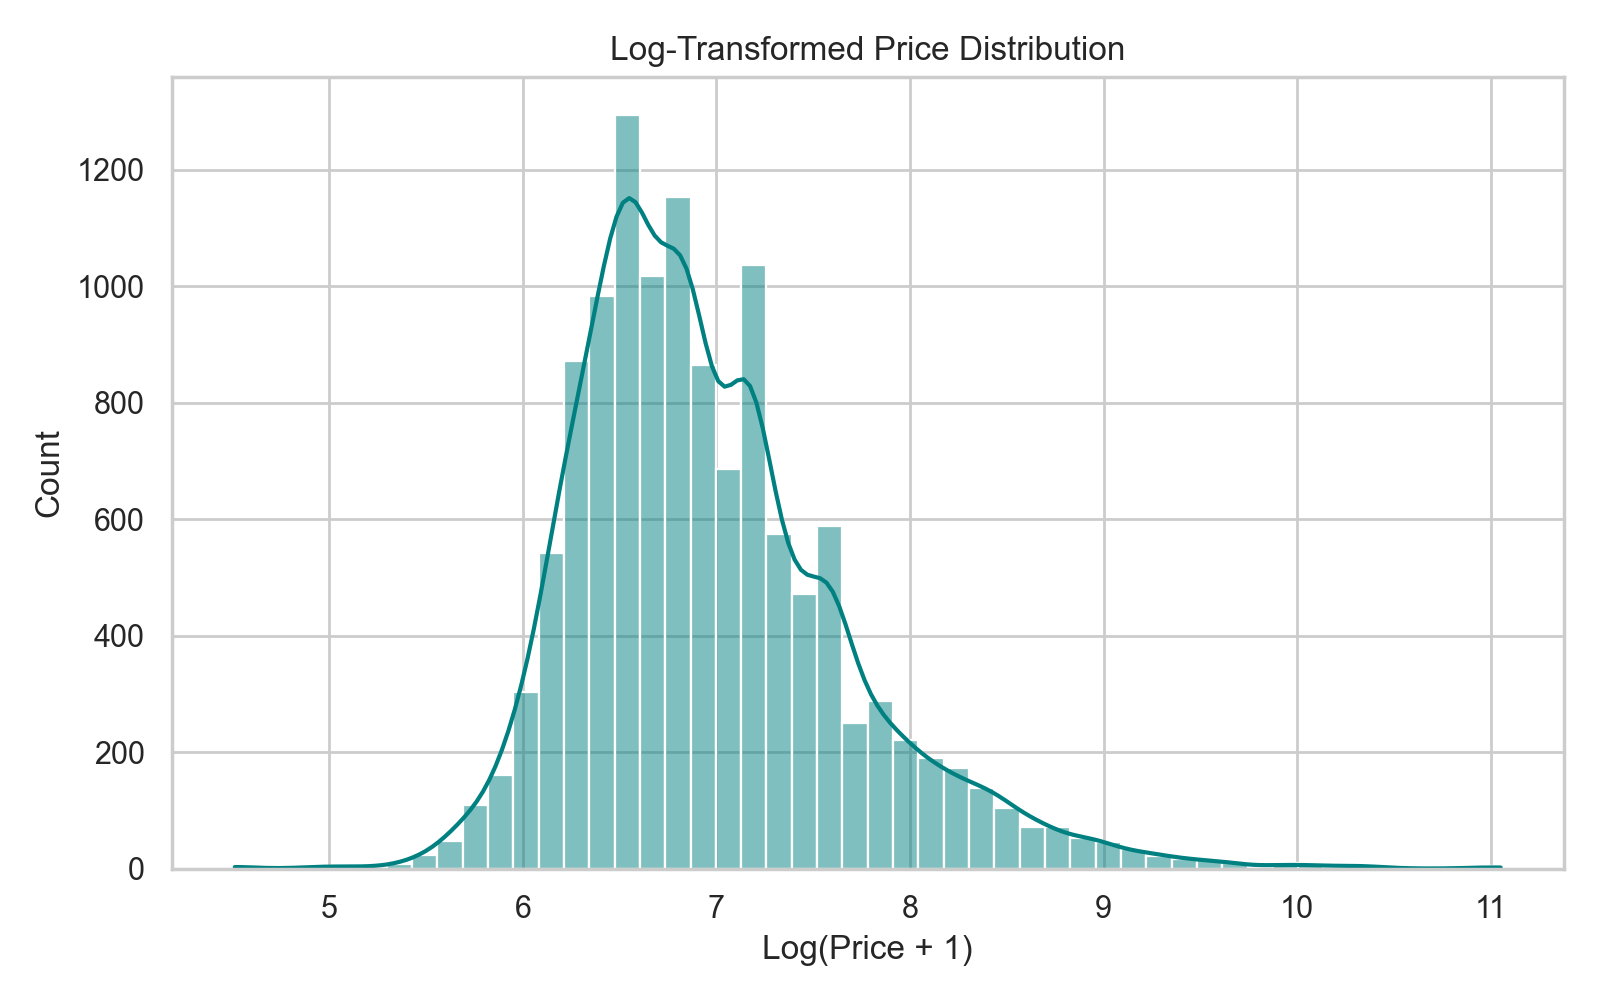
\includegraphics[width=0.75\textwidth]{imgs/log_price_distribution.png}}
{\fbox{\parbox[c][5cm][c]{0.75\textwidth}{\centering Missing image: \texttt{imgs/log\_price\_distribution.png}}}}
\caption{Separate histogram of the log-transformed price}
\label{fig:log_price_distribution}
\end{figure}

\begin{figure}[H]
\centering
\IfFileExists{imgs/log_price_by_gender.png}
{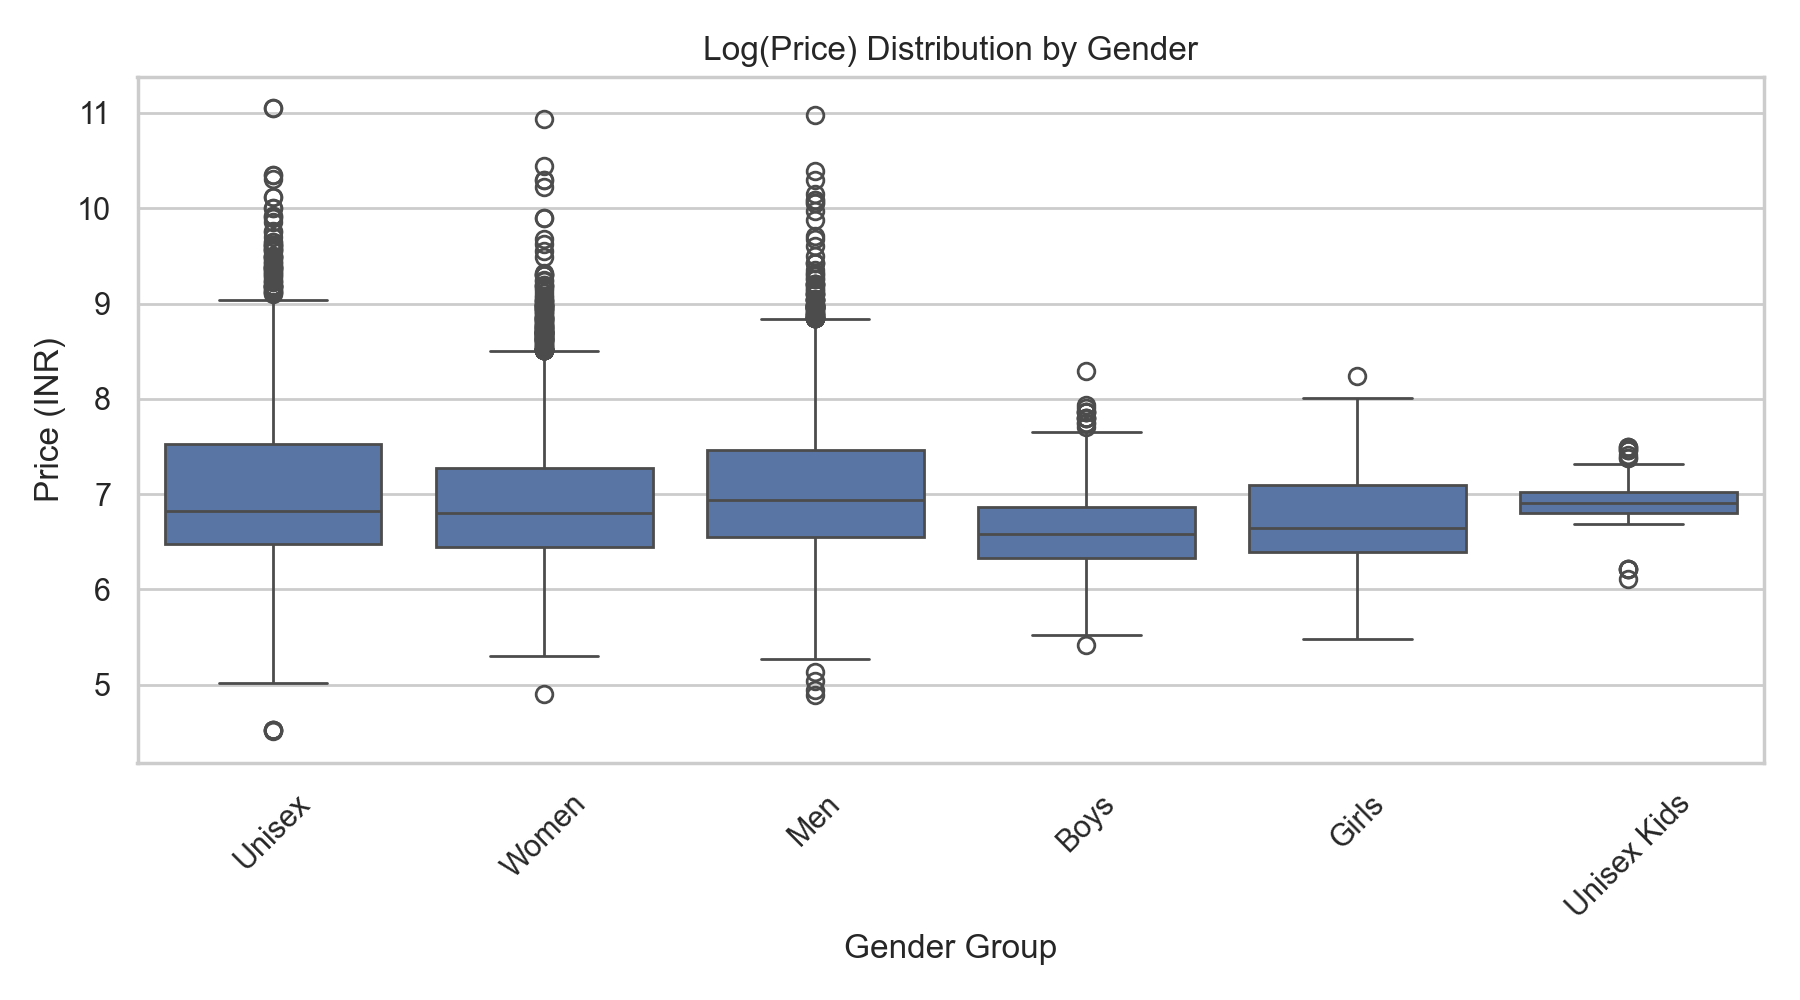
\includegraphics[width=0.8\textwidth]{imgs/log_price_by_gender.png}}
{\fbox{\parbox[c][5cm][c]{0.8\textwidth}{\centering Missing image: \texttt{imgs/log\_price\_by\_gender.png}}}}
\caption{Separate boxplot of log-transformed price by gender category}
\label{fig:log_price_by_gender}
\end{figure}

\section{Project Structure}

The project is organized into separate modules. This makes the code easier to read and also makes it possible to run the training pipeline and the web application separately.

\begin{lstlisting}[language=bash, caption={Main project files}]
main.py
src/config.py
src/data_loader.py
src/features.py
src/preprocessing.py
src/models.py
src/deep_learning.py
src/evaluation.py
src/pipeline.py
src/reporting.py
src/utils.py
app/app.py
data/test/app_test_products.txt
\end{lstlisting}

\begin{figure}[H]
\centering
\begin{tikzpicture}[
    node distance=1.6cm,
    every node/.style={draw, rounded corners, align=center, minimum width=3.7cm, minimum height=0.9cm},
    arrow/.style={-{Stealth[length=3mm]}, thick}
]
\node (data) {CSV data};
\node[below=of data] (features) {Cleaning and features};
\node[below=of features] (prep) {Preprocessing};
\node[below left=1.4cm and 1.4cm of prep] (models) {ML models};
\node[below right=1.4cm and 1.4cm of prep] (dl) {TensorFlow model};
\node[below=3.2cm of prep] (eval) {Evaluation};
\node[below=of eval] (app) {Streamlit app};

\draw[arrow] (data) -- (features);
\draw[arrow] (features) -- (prep);
\draw[arrow] (prep) -- (models);
\draw[arrow] (prep) -- (dl);
\draw[arrow] (models) -- (eval);
\draw[arrow] (dl) -- (eval);
\draw[arrow] (eval) -- (app);
\end{tikzpicture}
\caption{General data flow in the project}
\label{fig:pipeline}
\end{figure}

\section{Work Process}

\subsection{Loading the Data}

The data is loaded in the \texttt{src/data\_loader.py} module. The program checks whether the file exists and whether it contains all required columns. This is useful because data problems are detected early, before the training step starts.

\begin{lstlisting}[language=Python, caption={Checking required columns in the dataset}]
missing_columns = set(INPUT_COLUMNS + [TARGET_COLUMN]) - set(df.columns)
if missing_columns:
    raise ValueError(
        f"Dataset is missing required columns: {sorted(missing_columns)}"
    )
\end{lstlisting}

\subsection{Feature Engineering}

Additional features are created in the \texttt{src/features.py} module. The product description is used to calculate text length and a flag showing whether the description exists. The project also calculates brand name length and a simple color group, such as neutral, warm, cool, pastel, or metallic.

\begin{lstlisting}[language=Python, caption={Creating simple text features}]
output["Description"] = output["Description"].fillna("")
output["DescriptionLength"] = output["Description"].astype(str).str.len()
output["HasDescription"] = (output["DescriptionLength"] > 0).astype(int)
output["BrandNameLength"] = (
    output["ProductBrand"]
    .fillna("Unknown")
    .astype(str)
    .apply(infer_brand_length)
)
\end{lstlisting}

These features are simple, but they help the models use information that is not directly numerical. For example, a longer description may mean that the product is more detailed, more complex, or belongs to a higher price category.

\subsection{Preprocessing}

The preprocessing pipeline is built with \texttt{ColumnTransformer}. Different transformations are used for different column types:

\begin{itemize}
    \item \texttt{TargetEncoder} for the product brand,
    \item \texttt{OneHotEncoder} for gender category, primary color, and color group,
    \item \texttt{StandardScaler} for numerical features.
\end{itemize}

\begin{lstlisting}[language=Python, caption={Part of the preprocessing pipeline}]
transformer = ColumnTransformer([
    ("brand_target_encoding",
     TargetEncoder(smooth="auto", random_state=RANDOM_STATE),
     TARGET_ENCODING_COLUMNS),
    ("onehot_encoding",
     OneHotEncoder(handle_unknown="ignore", sparse_output=False),
     ONE_HOT_COLUMNS),
    ("numeric_scaling", numeric_pipeline, NUMERIC_FEATURES),
], remainder="drop")
\end{lstlisting}

The data was split into training and test sets using an 80/20 split. A fixed \texttt{RANDOM\_STATE} was used, so the results are reproducible.

\subsection{Models}

Several models were compared in the project. The project includes classic scikit-learn regression models and a simple deep learning model created with TensorFlow/Keras.

\begin{table}[H]
\centering
\begin{tabular}{|p{5cm}|p{8cm}|}
\hline
\textbf{Model} & \textbf{Short description} \\ \hline
KNN & predicts price based on similar products \\ \hline
SVM & regression model with an RBF kernel \\ \hline
RandomForest & ensemble of many decision trees \\ \hline
HistogramGradientBoosting & boosting model for tabular data \\ \hline
MLP & neural network from scikit-learn \\ \hline
TensorFlowDeepRegressor & custom Keras/TensorFlow model \\ \hline
\end{tabular}
\caption{Models used in the project}
\label{tab:models}
\end{table}

The main training pipeline is located in \texttt{src/pipeline.py}. It runs preprocessing, cross-validation, model training, test evaluation, and artifact saving.

\begin{lstlisting}[language=Python, caption={Running the full training pipeline}]
def main():
    print("Starting the ML pipeline execution")
    trained_models, preprocessor, report = run_training_pipeline()
    print("Training pipeline complete.")
\end{lstlisting}

\subsection{Streamlit Application}

After training, the application can be started with:

\begin{lstlisting}[language=bash, caption={Starting the Streamlit app}]
.\.venv\Scripts\python.exe -m streamlit run app/app.py
\end{lstlisting}

The application allows the user to choose a model, enter product data, and receive an estimated price. A small set of test products was also added in a text file:

\begin{lstlisting}[language=bash, caption={File with test products}]
data/test/app_test_products.txt
\end{lstlisting}

This makes the application easier to present. During a demonstration, a prepared product can be selected, and after clicking \texttt{Predict Price}, the app immediately shows the real price, predicted price, difference, and percentage error.

\section{Use Case Diagram}

\begin{figure}[H]
\centering
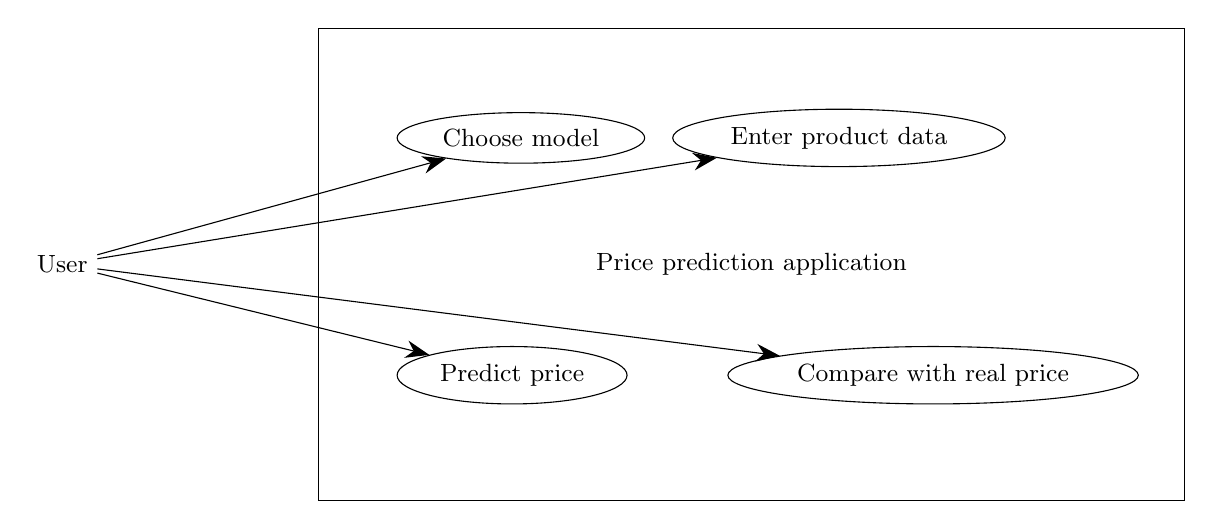
\begin{tikzpicture}[every node/.style={font=\small}, node distance=2cm]

\node[draw, rectangle, minimum width=11cm, minimum height=6cm] (system) {Price prediction application};

\node[draw, ellipse, right=1cm of system.north west, yshift=-1.4cm] (model) {Choose model};
\node[draw, ellipse, right=4.5cm of system.north west, yshift=-1.4cm] (data) {Enter product data};
\node[draw, ellipse, right=1cm of system.south west, yshift=1.6cm] (predict) {Predict price};
\node[draw, ellipse, right=5.2cm of system.south west, yshift=1.6cm] (compare) {Compare with real price};

\node[left=2.8cm of system] (user) {User};

\draw[-{Stealth[length=3mm]}] (user) -- (model);
\draw[-{Stealth[length=3mm]}] (user) -- (data);
\draw[-{Stealth[length=3mm]}] (user) -- (predict);
\draw[-{Stealth[length=3mm]}] (user) -- (compare);

\end{tikzpicture}
\caption{Use cases of the application}
\label{fig:usecase}
\end{figure}

\section{Results}

The final metrics are saved in:

\begin{lstlisting}[language=bash, caption={File with model metrics}]
reports/test_metrics.csv
\end{lstlisting}

Table~\ref{tab:results} shows the model results on the test set. MAE and RMSE are calculated in the logarithmic target scale, because the model was trained on \texttt{log1p(Price)}. In the application, the prediction is converted back and displayed in INR.

\begin{table}[H]
\centering
\begin{tabular}{|l|c|c|c|}
\hline
\textbf{Model} & \textbf{MAE} & \textbf{RMSE} & \textbf{R2} \\ \hline
RandomForest & 0.2597 & 0.3749 & 0.7181 \\ \hline
HistogramGradientBoosting & 0.2650 & 0.3776 & 0.7141 \\ \hline
TensorFlowDeepRegressor & 0.2819 & 0.3945 & 0.6879 \\ \hline
MLP & 0.2937 & 0.4072 & 0.6674 \\ \hline
SVM & 0.2929 & 0.4109 & 0.6614 \\ \hline
KNN & 0.2927 & 0.4194 & 0.6472 \\ \hline
\end{tabular}
\caption{Model comparison on the test set}
\label{tab:results}
\end{table}

The same results can also be presented visually. A bar chart makes it easier to compare models by the \texttt{R2} score. In the current version of the project, RandomForest and HistogramGradientBoosting achieved the strongest results, while the TensorFlow model was slightly weaker but still useful as a deep learning extension.

\begin{figure}[H]
\centering
\IfFileExists{imgs/baseline_models_r2.png}
{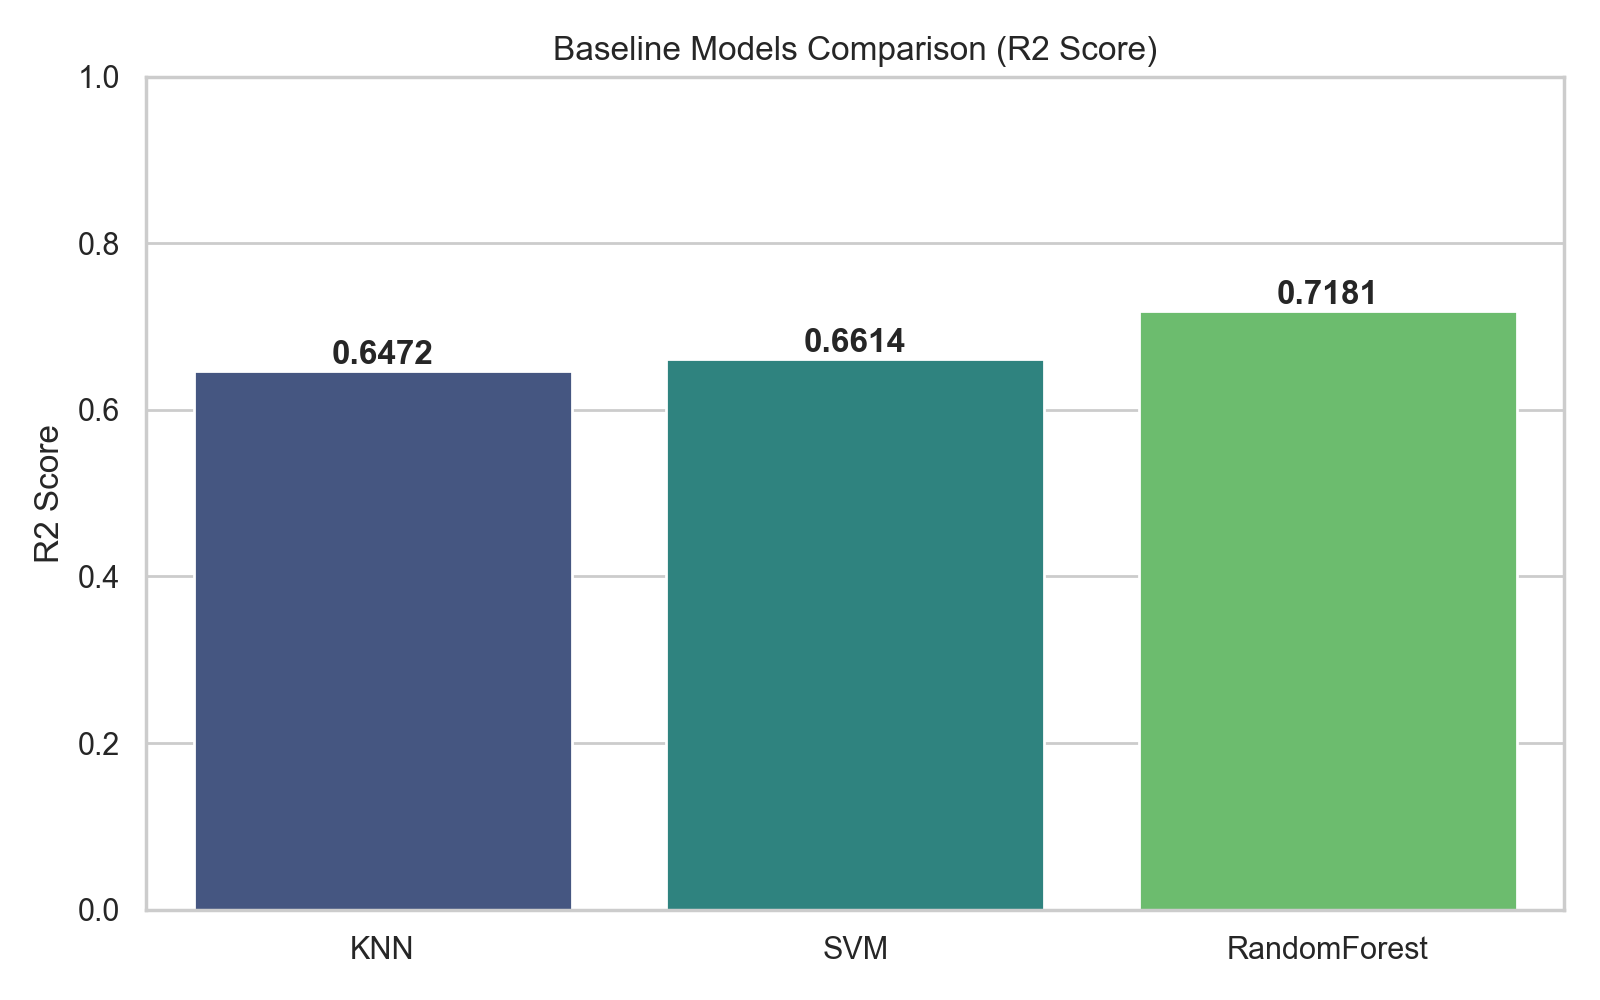
\includegraphics[width=0.8\textwidth]{imgs/baseline_models_r2.png}}
{\fbox{\parbox[c][6cm][c]{0.8\textwidth}{\centering Missing image: \texttt{imgs/baseline\_models\_r2.png}}}}
\caption{Baseline models comparison by R2 score}
\label{fig:baseline_models_r2}
\end{figure}

\begin{figure}[H]
\centering
\IfFileExists{imgs/baseline_vs_deep_learning.png}
{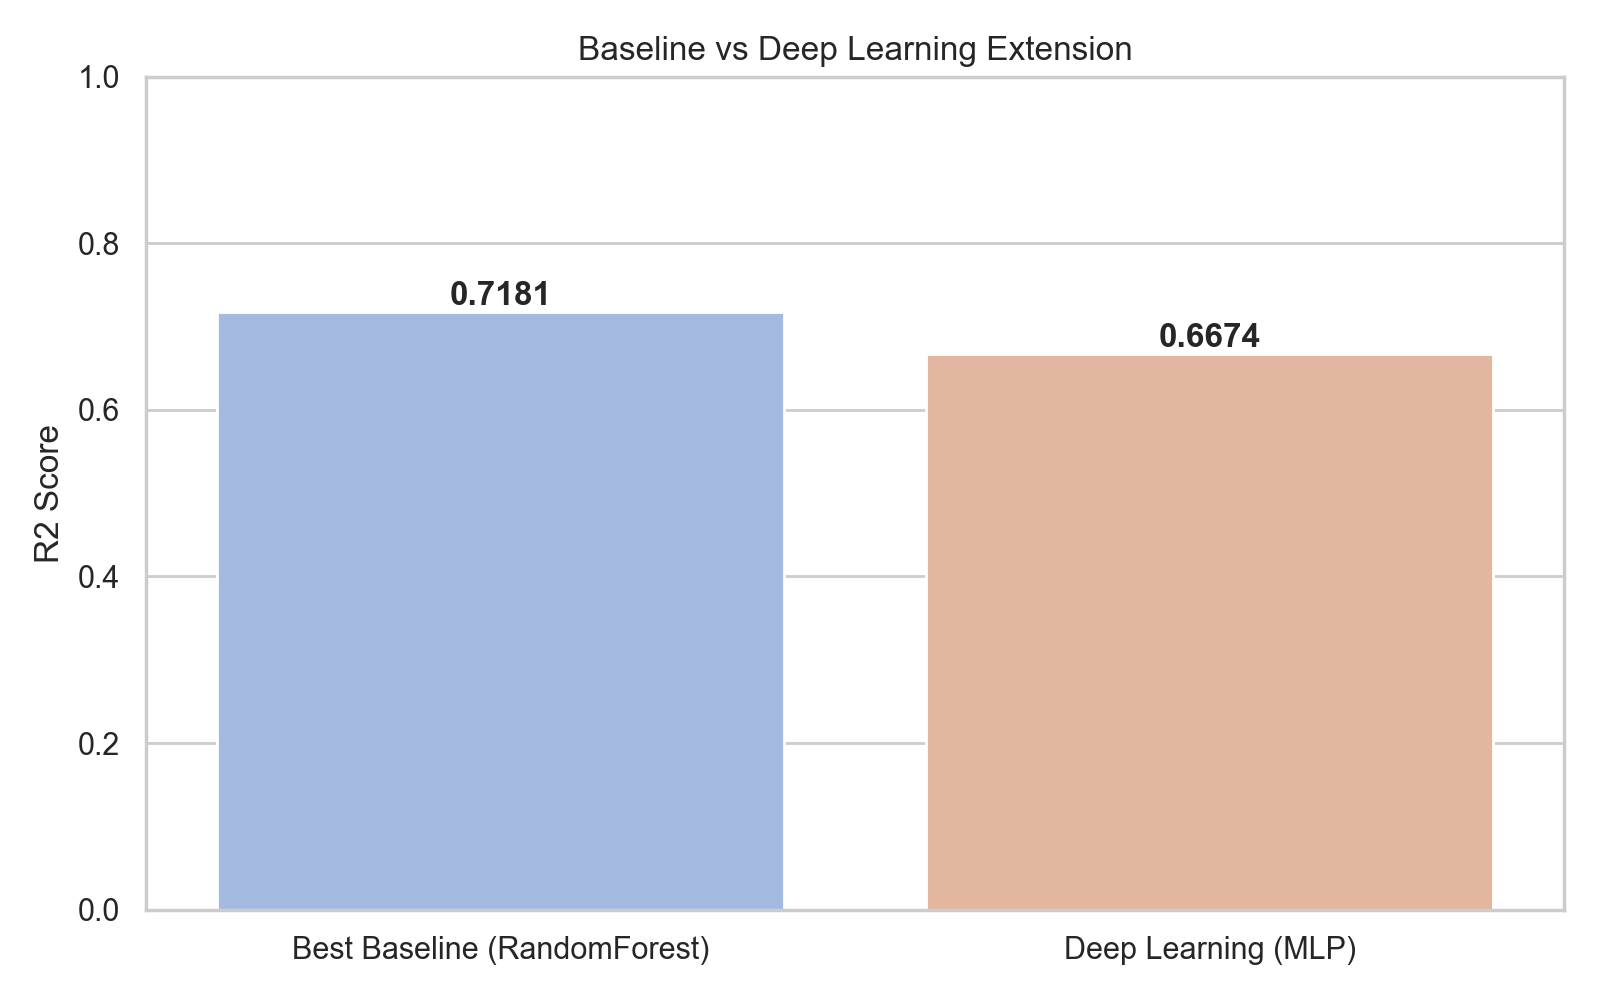
\includegraphics[width=0.8\textwidth]{imgs/baseline_vs_deep_learning.png}}
{\fbox{\parbox[c][6cm][c]{0.8\textwidth}{\centering Missing image: \texttt{imgs/baseline\_vs\_deep\_learning.png}}}}
\caption{Comparison between the best baseline model and the deep learning extension}
\label{fig:baseline_vs_deep_learning}
\end{figure}

The best model was RandomForest. Its \texttt{R2} score was about 0.718. This means that the model explains a large part of the price variation, but it is not perfect. This is expected in this type of task, because product price also depends on information that is not available in the dataset, such as material quality, current discounts, product collection, or brand positioning.

\section{Test Examples in the Application}

A separate file with test examples was added to the application. The examples were selected so that the KNN model gives predictions close to the real price. This is useful during presentation, because it quickly shows that the application works and that it can compare prediction with a real value.

\begin{table}[H]
\centering
\begin{tabular}{|p{4cm}|r|r|r|}
\hline
\textbf{Example} & \textbf{Real price} & \textbf{KNN prediction} & \textbf{Error} \\ \hline
Amraoo red dupatta & 599 & 602.12 & 0.52\% \\ \hline
MSC gold flats & 679 & 682.57 & 0.53\% \\ \hline
Indian Terrain polo & 764 & 759.81 & 0.55\% \\ \hline
Ed Hardy jeans & 1619 & 1627.52 & 0.53\% \\ \hline
Park Avenue blazer & 2699 & 2714.12 & 0.56\% \\ \hline
Kazo navy jeggings & 895 & 889.63 & 0.60\% \\ \hline
\end{tabular}
\caption{Examples used for a quick application demonstration}
\label{tab:test_examples}
\end{table}

\section{Running the Project}

The project can be run locally from the root directory. First, the virtual environment should be activated and dependencies should be installed.

\begin{lstlisting}[language=bash, caption={Installing dependencies}]
.\.venv\Scripts\Activate.ps1
pip install -r requirements.txt
\end{lstlisting}

Model training:

\begin{lstlisting}[language=bash, caption={Training the models}]
.\.venv\Scripts\python.exe main.py
\end{lstlisting}

Starting the application:

\begin{lstlisting}[language=bash, caption={Starting the application}]
.\.venv\Scripts\python.exe -m streamlit run app/app.py
\end{lstlisting}

\section{Problems and Fixes During Development}

Several practical issues appeared during development. The first one was related to the \texttt{ColorGroup} column. This feature was created in \texttt{features.py}, but at first it was not passed to the model input. This caused an error during preprocessing. The issue was fixed by adding the \texttt{MODEL\_FEATURE\_COLUMNS} list.

The second issue was related to running the project on Windows. The terminal showed that the \texttt{.venv} environment was active, but sometimes the \texttt{python} command still pointed to the Microsoft Store Python installation. Because of that, the instructions use the explicit path to the Python interpreter inside the virtual environment:

\begin{lstlisting}[language=bash, caption={Safe execution using Python from the virtual environment}]
.\.venv\Scripts\python.exe main.py
\end{lstlisting}

The third issue was an old model file named \texttt{mlp\_neuralnetwork.pkl}. The file is still in the model directory, but the application does not show it in the model selection list. The list is now built using the current training report, so only valid and current models are shown.

\section{Conclusions}

The project meets the main goal. The data is loaded and prepared automatically, models are trained in one pipeline, and the results are saved to reports. RandomForest achieved the best overall result, but the application also allows checking other models, including the TensorFlow model.

The most important part of the project is that it is not only an experiment in a notebook. A full path from raw data to a working application was created. The user can select a prepared test example or enter custom product data. After clicking the prediction button, the application shows the estimated price and, for test examples, compares it with the real product price.

The model should not be treated as a professional commercial pricing tool, because the dataset does not contain all factors that influence price. Still, the results are reasonable, and the project shows the complete process of building a simple predictive system: data preparation, model training, evaluation, and deployment in a small web application.

\section{Appendix: Plot and Table Code}

This section contains the code used to prepare the plots for the report. The images are saved into the \texttt{imgs/} folder and can be uploaded to Overleaf with the same filenames.

\begin{lstlisting}[language=Python, caption={Generating exploratory plots}]
import numpy as np
import pandas as pd
import matplotlib.pyplot as plt
import seaborn as sns

df = pd.read_csv("data/raw/myntra_products_catalog.csv")
sns.set_theme(style="whitegrid")
log_price = np.log1p(df["Price (INR)"])
plot_df = df.copy()
plot_df["LogPrice"] = log_price

fig, axes = plt.subplots(1, 2, figsize=(16, 5))
sns.histplot(log_price, bins=50, kde=True, color="teal", ax=axes[0])
axes[0].set_title("Log-Transformed Price Distribution")
axes[0].set_xlabel("Log(Price + 1)")
axes[0].set_ylabel("Count")
sns.boxplot(data=plot_df, x="Gender", y="LogPrice", ax=axes[1])
axes[1].set_title("Log(Price) Distribution by Gender")
axes[1].set_xlabel("Gender Group")
axes[1].set_ylabel("Price (INR)")
axes[1].tick_params(axis="x", rotation=45)
fig.tight_layout()
fig.savefig("imgs/eda_price_plots.png", dpi=200)

fig, ax = plt.subplots(figsize=(8, 5))
sns.histplot(log_price, bins=50, kde=True, color="teal", ax=ax)
ax.set_title("Log-Transformed Price Distribution")
ax.set_xlabel("Log(Price + 1)")
ax.set_ylabel("Count")
fig.tight_layout()
fig.savefig("imgs/log_price_distribution.png", dpi=200)

fig, ax = plt.subplots(figsize=(9, 5))
sns.boxplot(data=plot_df, x="Gender", y="LogPrice", ax=ax)
ax.set_title("Log(Price) Distribution by Gender")
ax.set_xlabel("Gender Group")
ax.set_ylabel("Price (INR)")
ax.tick_params(axis="x", rotation=45)
fig.tight_layout()
fig.savefig("imgs/log_price_by_gender.png", dpi=200)
\end{lstlisting}

\begin{lstlisting}[language=Python, caption={Generating model comparison plots from test\_metrics.csv}]
import pandas as pd
import matplotlib.pyplot as plt
import seaborn as sns

metrics = pd.read_csv("reports/test_metrics.csv")
sns.set_theme(style="whitegrid")

plt.figure(figsize=(8, 5))
baseline = metrics[metrics["model"].isin(["KNN", "SVM", "RandomForest"])]
ax = sns.barplot(data=baseline, x="model", y="R2", palette="viridis")
plt.title("Baseline Models Comparison (R2 Score)")
plt.xlabel("")
plt.ylabel("R2 Score")
plt.ylim(0, 1)
for container in ax.containers:
    ax.bar_label(container, fmt="%.4f", fontweight="bold")
plt.tight_layout()
plt.savefig("imgs/baseline_models_r2.png", dpi=200)

plt.figure(figsize=(8, 5))
comparison = pd.DataFrame({
    "model": ["Best Baseline (RandomForest)", "Deep Learning (MLP)"],
    "R2": [
        metrics.loc[metrics["model"] == "RandomForest", "R2"].iloc[0],
        metrics.loc[metrics["model"] == "MLP", "R2"].iloc[0],
    ],
})
ax = sns.barplot(data=comparison, x="model", y="R2", palette=["#9bb7eb", "#efb293"])
plt.title("Baseline vs Deep Learning Extension")
plt.xlabel("")
plt.ylabel("R2 Score")
plt.ylim(0, 1)
for container in ax.containers:
    ax.bar_label(container, fmt="%.4f", fontweight="bold")
plt.tight_layout()
plt.savefig("imgs/baseline_vs_deep_learning.png", dpi=200)
\end{lstlisting}

The table with final model metrics is stored in the project as:

\begin{lstlisting}[language=bash, caption={Metrics CSV used for the report table}]
reports/test_metrics.csv
\end{lstlisting}

% Bibliography

\newpage
\begin{thebibliography}{9}

\bibitem{sklearn}
Scikit-learn documentation, \url{https://scikit-learn.org/}

\bibitem{tensorflow}
TensorFlow documentation, \url{https://www.tensorflow.org/}

\bibitem{streamlit}
Streamlit documentation, \url{https://streamlit.io/}

\bibitem{pandas}
Pandas documentation, \url{https://pandas.pydata.org/}

\end{thebibliography}

\end{document}
